%Empieza configuracion de capitulo
\setstretch{1.0}
\titleformat{\chapter}[block]{\Large\bfseries}{CHAPTER \Huge\thechapter\vspace{25 pt}}{0 pt}{\\\fontsize{26}{36}\selectfont}
\titlespacing{\chapter}{0 pt}{30 pt}{50 pt}[0 pt]
\titleformat{\section}{\Large\bfseries}{\thesection}{0 pt}{\hspace{30 pt}}
\titleformat{\subsection}{\large\bfseries}{\thesubsection}{0 pt}{\hspace{30 pt}}
\pagestyle{fancy}
\fancyhead[LO,LE]{\footnotesize\emph{\leftmark}}
\fancyhead[RO,RE]{\thepage}
\fancyfoot[CO,CE]{}
%Termina configuracion de capitulo

\chapter{Theoretical Framework}
\setstretch{1.5} %Regresa el interlineado a 1.5

\normalsize
\noindent

This is a new topic that will require quite a few topics to fully understand
further experiments and why we decided to do them. We will try to cover as much
of the topics needed to fully understand the problem and the proposed
solution. However will not cover deep topics as Operating Systems architecture
nor parallel programming concepts.


\section{The need of parallel computing}
\noindent

Computer technology has made incredible progress in the roughly 60 years since
the first general-purpose electronic computer was created. Today, less than 500
USD will purchase a personal computer that has more performance, more main
memory, and more disk storage than a computer bought in 1985 for 1 million
dollars. This rapid improvement has come both from advances in the technology
used to build computers and from innovation in computer design. \cite{Hennessy}

As we have seen it was around the years 2003 to 2005 that a dramatic change
seized the semiconductor industry and the manufactures of processors. The
increasing of computing performance in processors, based on simply screwing up
the clock frequency, could not longer be holded. The answer of the industry to
that development, in order to still meet Moore's law, was the shifting to real
parallelism by doubling the number of processors on one chip die. This was the
birth of the multi-core area. 

Where do we find parallelism  examples in embedded systems? A good example are
automotive applications multi-core technology in combination with a broadband
efficient network system offers the possibility to save components too by
migrating functionality that is now distributed among a quite large number of
compute devices to fewer cores.


\section{Distributed Systems}
\noindent

We define a distributed system as one in which hardware or software components
located at networked computers communicate and coordinate their actions only by
passing messages. This simple definition covers the entire range of systems in
which networked computers can usefully be deployed.

Computers that are connected by a network may be spatially separated by any
distance. They may be on separate continents, in the same building or in the
same room. Our definition of distributed systems has the following significant
consequences:


\begin{enumerate}

\item \textbf{Concurrency:}
In a network of computers, concurrent program execution is the norm. I can
do my work on my computer while you do your work on yours, sharing resources
such as web pages or files when necessary. The capacity of the system to handle
shared resources can be increased by adding more resources (for example.
computers) to the network.

\item \textbf{No global clock:}
When programs need to cooperate they coordinate their actions
by exchanging messages. Close coordination often depends on a shared idea of
the time at which the programs actions occur. But it turns out that there are
limits to the accuracy with which the computers in a network can synchronize
their clocks there is no single global notion of the correct time. This is a
direct consequence of the fact that the only communication is by sending
messages through a network.

\item \textbf{Independent failures:}
All computer systems can fail, and it is the
responsibility of system designers to plan for the consequences of possible
failures. Distributed systems can fail in new ways. Faults in the network
result in the isolation of the computers that are connected to it, but that
doesn't mean that they stop running. In fact, the programs on them may not be
able to detect whether the network has failed or has become unusually slow.
Similarly, the failure of a computer, or the unexpected termination of a
program somewhere in the system (a crash), is not immediately made known to the
other components with which it communicates. Each component of the system can
fail independently, leaving the others still running.

\end{enumerate}


Each one these characteristics is also present in a modern IoT system. As we can
see in (figure~\ref{fig:3.1}). As we can see these three characteristics of a
distributed system are also present in an IoT system. 

\begin{figure}[H]
\centering
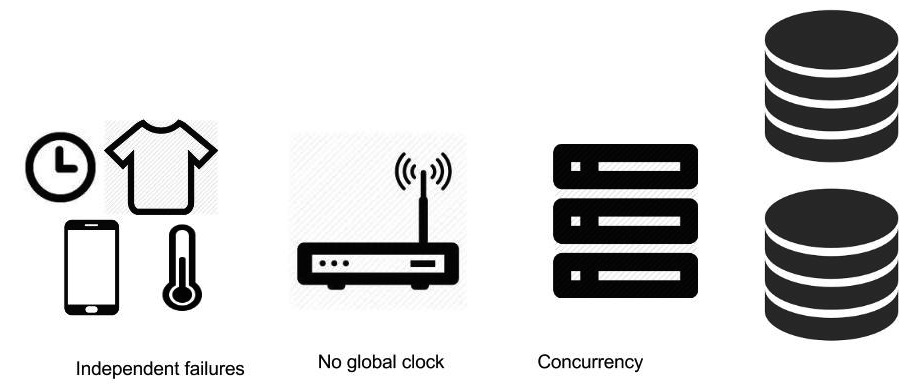
\includegraphics[width=0.75\textwidth]{images/IoT_distributed.jpg}
\caption{IoT system as a distributed system}
\label{fig:3.1}
\end{figure}


\begin{enumerate}
\item \textbf{Concurrency}
In an IoT system there are multiple systems trying to use the same resource.
For example all the IoT devices are trying to access the same data base or the
even the same access's point. All of them are fighting for similar resources , a
good IoT design need to schedule the use of the limited resources in an efficient
way.

\item \textbf{No global clock}
None of the systems in an IoT network (either sensors or processing devices)
have the same clock. They have to use a message base mechanism to communicate
each other. 

\item \textbf{Independent failures}
In a regular IoT network multiple systems could fail (either sensors,
processing devices or one of the data centers) and despite of that all the
others should keep working without any problem. 

All these characteristics enforce the idea that the nature of an IoT system is
being treated as a distributed system. With this main idea is much more simple
to adapt the solutions of the distributed systems into our embedded distributed
system.

\end{enumerate}

\section{Embedded Linux systems}

Computers are everywhere , this fact, of course, is not a surprise to anyone 
who hasn't been living in a cave during the past 25 years or so. And you
probably know that computers aren't just on our desktops, in our kitchens, and, 
increasingly, in our living rooms holding our music collections. They're also 
in our microwave ovens, our regular ovens, our cellphones, and our portable 
digital music players.

Until not too long time ago, embedded systems were not very powerful, and they
ran special-purpose, proprietary operating systems that were very different
from industry-standard ones. (Plus, they were much harder to develop for.)
Today, embedded computers are as powerful as, if not more than, a modern home
computer. (Consider the high-end gaming consoles, for example.)

Along with this power comes the capability to run a full-fledged operating
system such as Linux. Using a system such as Linux for an embedded product
makes a lot of sense. A large community of developers are making it possible.
The development environment and the deployment environment can be surprisingly
similar, which makes your life as a developer much easier. And you have both
the security of a protected address space that a virtual memory-based system
gives you, and the power and flexibility of a multiuser, multiprocessor system.
That's a good deal all around. For this reason, companies all over the world
are using Linux on many devices

In the beginning embedded systems were most commonly resource constrained
compared to the typical desktop PC. Embedded systems often had limited memory,
small or no hard drives, and sometimes no external network connectivity.
Frequently, the only user interface was a serial port and some LED's. But today
there has been a change in the last point: external network connectivity.

The internet of things is the evolution of the embedded world in terms of
connectivity. The IoT systems keep being resource constrained but with the
capability to be connected to an internet network where to send the data to
external servers (where it will be analyzed, stored and presented in a web base
user interface to the end user)

In this new world the advantages (flexibility and scalability) of using Linux
as the core of the OS Embedded Distributions turn out to make a nightmare for
the embedded developers with too many options and no standard work to re use.
In the end, the developer ended with a ''Frankenstein'' embedded Linux
distribution with very low maintainability and robustness. In 2010 there was a
change in the industry of embedded systems, the announce of a project to solve
these kind of problems: The Yocto project.

\section{The Yocto project}
\noindent
The Yocto Project is an open source collaboration project that provides
templates, tools and methods to help you create custom Linux-based systems for
embedded products regardless of the hardware architecture. It was founded in
2010 as a collaboration among many hardware manufacturers, open-source
operating systems vendors, and electronics companies to bring some order to the
chaos of embedded Linux development.\cite{yocto-project}

As an open source project, the Yocto Project operates with a hierarchical
governance structure based on meritocracy and managed by its chief architect,
Richard Purdie, a Linux Foundation fellow. This enables the project to remain
independent of any one of its member organizations, who participate in various
ways and provide resources to the project.

Why to use the Yocto Project? It's a complete embedded Linux development
environment with tools, meta-data, and documentation. The
free tools are easy to get started with, powerful to work with (including
emulation environments, debuggers, an Application Toolkit Generator, etc.) and
they allow projects to be carried forward over time without causing you to loose
optimizations and investments made during the project's prototype phase. The
Yocto Project fosters community adoption of this open source technology
allowing its users to focus on their specific product features and development.

The Yocto Project through the Poky build tool provides an open source
development environment (figure~\ref{fig:3.1}). targeting the ARM, MIPS,
Power-PC and x86 architectures for a variety of platforms including x86-64 and
emulated ones.  You can use components from the Yocto Project to design,
develop, build, debug, simulate, and test the complete software stack using
Linux, the X Window System, GNOME Mobile-based application frameworks, and Qt
frameworks. 

\begin{figure}[H]
\centering
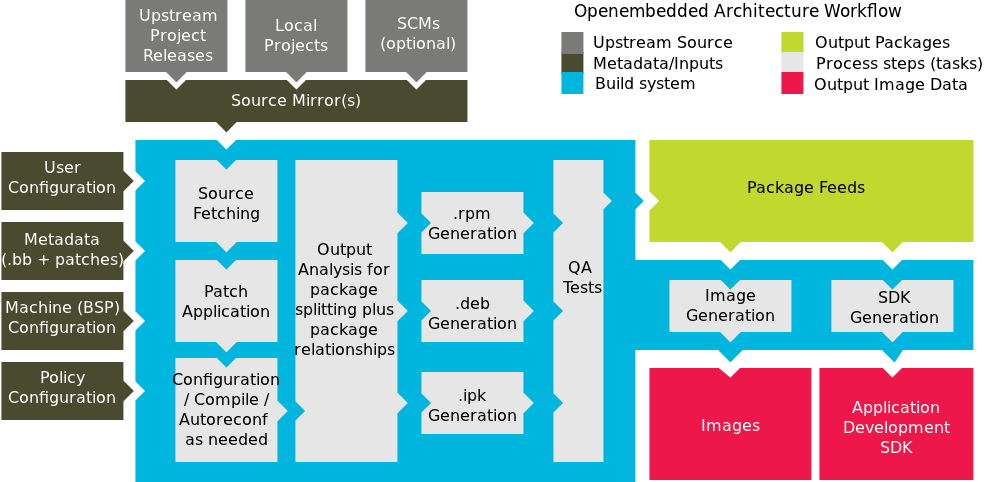
\includegraphics[width=0.75\textwidth]{images/yocto-environment.png}
\caption{The Yocto Project Development Environment}
\label{fig:3.2}
\end{figure}

For complete information on the Yocto Project, you should check out the Yocto
Project website\cite{yocto-project}. As you can see the Yocto project will play
an important role in the IoT world. If we want to develop a solution standard
for multiple platforms we might adapt it for the Yocto project. If we do this
our solution will be deployable into multiple IoT devices due to the bast
amount of platforms ( sensors and processing devices ) that use the Yocto
project everyday.

\section{Power and Performance}

\noindent
When we say one computer is faster than another , what do we mean? The user
of a desktop computer may say a computer is faster when a program runs in less
time, while an Amazon.com administrator may say a computer is faster when it
completes more transactions per hour. The computer user is interested in 
reducing response time (the time between the start and the completion of an 
event) also referred to as execution time. The administrator of a large data 
processing center may be interested in increasing throughput (the total amount 
of work done in a given time.) 

In comparing design alternatives, we often want to relate the performance of
two different computers, say, X and Y. The phrase ''X is faster than Y'' is
used here to mean that the response time or execution time is lower on X than
on Y for the given task. In particular, ''X is n times faster than ''  will
mean

Since execution time is the reciprocal of performance, the following
relationship holds:

The phrase “the throughput of X is 1.3 times higher than Y” signifies here that
the number of tasks completed per unit time on computer X is 1.3 times the
number completed on Y.

The power and performance efficiency of our embedded distributed system is very
important. If we can  make the system process more data with less number
of systems more IoT applications will consider use this approach for their
solutions.

\clearpage
